\section{O algoritmo SHA-3}

O \textbf{SHA-3} é um algoritmo de \textit{hash} que foi escolhido em uma
competição do \textbf{NIST}, o instituto de padrões e normas dos Estados
Unidos, para criar uma função mais segura que as anteriores. Como os padrões
MD5 e SHA-0 haviam sido quebrados e o SHA-1 já possuía ataques teóricos, e com
o fato de que o SHA-2 era bastante semelhante ao SHA-1 e possíveis ataques
poderiam enfraquecer ambos os algoritmos, o NIST buscou um algoritmo com uma
estrutura diferente que pudesse resistir e substituí-los nesse caso.

O algoritmo escolhido como SHA-3 é baseado na família de funções esponja
\textbf{Keccak}, mais especificamente na variante com 1600 bits de largura da
função de permutação~\cite{fips:2015}.

O Keccak segue a a estrutura dos algoritmos de \textit{hash} comuns, onde os
blocos $P$ da mensagem a ser cifrada vão sendo concatenados alternadamente com
aplicações de uma função de transformação $f$, de forma que a passagem $i$
tenha o seguinte formato:

\begin{center}
        $S_{i} = f(S_{i-1} \oplus P_{i})$
\end{center}

Adicionalmente, explorando essa forma genérica de algoritmos de hash e de uma
função $f$ específica, o Keccak permite que tanto sua entrada quanto sua saída
tenham um tamanho variável, e possa ser usado não somente para verificar a
integridade de uma mensagem, mas como um gerador de números pseudoaleatórios,
além de outras aplicações.

\subsection{Funções esponja}

Funções esponja são uma classe de funções que recebem uma entrada de tamanho
finito qualquer e produzem uma saída com outro tamanho qualquer desejado, sendo
definidas por três parâmetros: um estado $S$, que contém $b$ bits; uma função
$f$ que permuta ou transforma o estado $S$; e uma função de \textit{padding}
$P$~\cite{noekeon:2011}.

Na inicialização, a função $P$ é aplicada na entrada $M$ e dividida em blocos
de $r$ bits. Os $b$ bits do estado $S$ são zerados. A construção da esponja se
dá em duas fases, chamadas de absorção e compressão.

O tamanho $r$ também é chamado de \textit{bitrate}, porque representa a
quantidade de bits da entrada que são consumidos em cada iteração da função
esponja, e o tamanho $c = |S| - r$ é chamado de capacidade, e representa o
nível de segurança atingido pela variante da função - SHA-3, $r + c = 1600$.

Aumentar o tamanho de $r$ para tornar o algoritmo mais rápido (gerando o
\textit{hash} com menos iterações) diminui, portanto, o nível de segurança do
\textit{hash} gerado, porém um nível muito alto de segurança implica numa
quantidade muito alta de iterações para gerar o \textit{hash}.

\subsection{Absorção e compressão}

Na fase de absorção, cada bloco $P$ de $r$ bits é combinado com os primeiros
$r$ bits, com os restantes $c$ bits preenchidos com zero, do estado $S$ com
\texttt{xor} e é aplicada a função $f$ no resultado, ou seja,
$S_{i} = f(S_{i-1} \oplus P_{i} \| 0^{c})$.

Ao final de todas as iterações, ou seja, após a mensagem $M$ ser completamente
consumida pela absorção da esponja, a saída da função $f$ será o \textit{hash}
gerado.

Na fase de compressão, os primeiros $r$ bits do estado $S$ são retornados, e
caso mais bits sejam desejados, se aplica novamente a função $f$ em $S$ para
transformar o estado. A representação gráfica dessas fases pode ser vista na
figura~\ref{fig:sponge}.

\begin{figure}[ht]
    \centering
    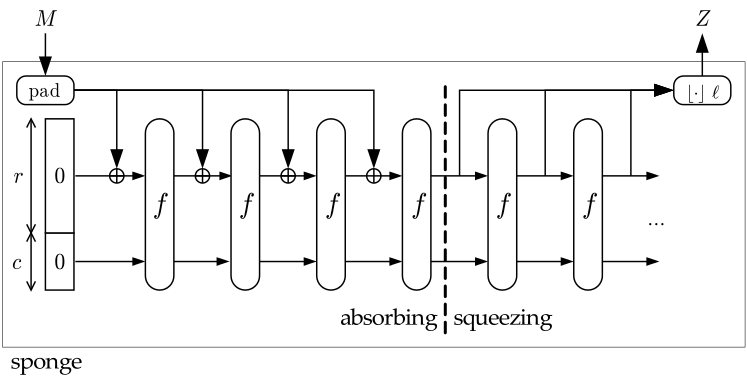
\includegraphics{images/esponja.png}
    \caption{Diagrama de uma função esponja}
    \label{fig:sponge}
\end{figure}

Os últimos $c$ bits não são diretamente afetados pela entrada $M$ e não são
produzidos como saída da função. A função esponja produz uma quantidade
indefinida de bits aleatórios.

\subsection{Função Keccak}

A função de compressão Keccak ($f$, não confundir com a compressão da esponja)
é uma função que tem como entrada um valor $S$ de $b$ \textit{bits}, de
$r + c = 1600$ bits no SHA-3. Esse valor $S$ é então dividido em uma matriz $A$
$5 \times 5$, onde cada célula contém 64 \textit{bits}. As posições dessa
matriz possuem índices $x$ (linha), $y$ (coluna) e $z$ (célula).

Uma vez criado esse estado interno, a função aplica 24 rodadas de processamento
$R_{i}$ que levam em consideração o resultado da rodada anterior e uma
constante $RC_{i}$

Cada uma das rodadas $R$ consiste na composição de cinco funções e pode ser
expressa pela seguinte função:

\begin{center}
    $R_{i} = \iota \circ \chi \circ \pi \circ \rho \circ \theta$
\end{center}

As funções possuem a seguinte fórmula:

\begin{itemize}
    \setlength\itemsep{1em}

    \item $\theta(M[x, y, z]) = M[x, y, z] \oplus \sum\limits_{y'=0}^{4}M[x-1, y', z] \oplus \sum\limits_{y'=0}^{4}M[x+1, y', z-1]$ \newline
        Este passo é uma função de substituição que utiliza bits de células adjacentes, cada \textit{bit} dependento de outros 11, o que provê boa difusão, o que é importante para o efeito avalanche.

    \item $\rho(M[x, y, z]) = \begin{cases}
            M[x, y, z], \mbox{se } x=y=0 \\
            M[x, y, z - \frac{(t+1)(t+2)}{2}] \mid 0 \leq t < 24 \land \begin{pmatrix}0 & 1 \\ 2 & 3\end{pmatrix} \begin{pmatrix}0 \\ 1\end{pmatrix} = \begin{pmatrix}x \\ y\end{pmatrix}\mbox{ em } GF(5)
        \end{cases}$ \newline
        Função de espalhamento dos \textit{bits} de uma célula para auxiliar na difusão de forma mais rápida.

    \item $\pi(M[x, y]) = M[x', y'], \mid \begin{pmatrix}x \\ y\end{pmatrix}\begin{pmatrix}0 & 1 \\ 2 & 3\end{pmatrix} = \begin{pmatrix}x' \\ y'\end{pmatrix}$ \newline
        Outra função de espalhamento dos \textit{bits}, mas entre células diferentes.

    \item $\chi(M[x, y, z]) = M[x, y, z] \oplus (\neg{M}[x+1, y, z] \land M[x+2, y, z])$ \newline
        Esta função é uma substituição baseada no valor atual do bit e dos próximos 2 bits, tornando o Keccak uma função não-linear, característica que os outros passos não provêm.

    \item $\iota(M[x, y, z]) = M[x, y, z] \oplus RC_{i}$, onde $RC_{i}$ é a constante da rodada citada acima e diferente para cada rodada $i$. \newline
        Função de substituição baseada em uma tabela e que envolve uma constante que é diferente a cada passo da função aplicado.
\end{itemize}

\subsection{Parâmetros do SHA-3}

O SHA-3 define um algoritmo padrão para uso com parâmetros diferentes,
dependendo do nível de segurança e tamanho de \textit{bits} desejados na saída.
A tabela abaixo enumera os parâmetros normalmente utilizados com o SHA-3:

\begin{center}
    \renewcommand{\arraystretch}{1.2}
    \newcolumntype{M}[1]{>{\centering\arraybackslash}m{#1}}
    \begin{tabular}{ M{2.4cm} | M{2.4cm} | M{2.4cm} | M{2.4cm} | M{2.4cm} }
        Tamanho do valor de \textit{hash} & Tamanho do bloco $r$ & Capacidade $c$ & Resistência a colisão & Resistência a segunda pré-imagem \\ \hline
        224 & 1152 & 448 & $2^{112}$ & $2^{224}$ \\ \hline
        256 & 1088 & 512 & $2^{128}$ & $2^{256}$ \\ \hline
        384 & 832 & 768 & $2^{192}$ & $2^{384}$ \\ \hline
        512 & 576 & 1024 & $2^{256}$ & $2^{512}$
    \end{tabular}
\end{center}

Como visto nas seções anteriores, quanto maior o tamanho do bloco (ou
\textit{bitrate}), maior a vazão de \textit{bits}, porém menor a segurança do
SHA-3. Isto é evidente nos valores de resistência a colisão e à segunda
pré-imagem, que mostram que quanto menor é o \textit{bitrate}, maior é a
resistência. Observe também que, para os tamanhos de valor de \textit{hash} da
tabela acima, não há necessidade de se usar a fase de espremer a esponja do
algoritmo do SHA-3, pois é sempre menor que nestes casos.
